\section{Analysemuster}\label{sec:analysemuster}

\subsection*{Muster}
Im Software Engineering versteht man unter dem Begriff \textit{Muster} (\textit{Pattern}) \textbf{vorgefertigte Lösungsschablonen für verallgemeinerte Probleme}.\\

\noindent
Bei der Entwicklung tauchen häufig ähnliche Probleme auf, bei denen sich auch die Art der Lösung entsprechend ähnelt.\\

\noindent
Die Beschreibung der verallgemeinerten Probleme und Lösungen auf eine \textbf{formalisierte Weise} nennt man \textbf{Muster}.\\

\noindent
Muster müssen zur Anwendung auf ein konkretes Problem \textit{konkretisiert} werden.\\

\noindent
Im Bereich des Software Engineerings gibt es Muster für \textbf{Analyse}, \textbf{Architektur}, \textbf{Entwurf}.

\subsection*{Vorteile}

\begin{itemize}
    \item es stehen \textbf{bewährte Standardlösungen} zur Verfügung
    \item Verwendung bereits bewährter Lösungen ist oft \textbf{schneller und besser} als selbstentwickelte neue Lösungen
    \item Muster helfen bei der \textbf{Kommunikation}
\end{itemize}


\subsection*{Standardisierte Beschreibung}

\begin{itemize}
    \item Beschreibung des Problems in seinem Kontext
    \item Lösung
    \item Beispiele
    \item Gegebenenfalls Antimuster
\end{itemize}

\noindent
Eine Auswahl wichtigster Analysemuster in der o.a standardisierten Beschreibung findet sich in~\cite[22 ff.]{Wed09b} und wird im Folgenden verkürzt wiedergegeben.

\subsection{Exemplartyp (Abstraction - Occurence)}

\subsubsection*{Problem}
\begin{itemize}
    \item Objekte einer Klasse ähneln sich untereinander und tragen gemeinsamen, gleiche Informationen oder besitzen gleiches  Verhalten, unterscheiden sich aber wesentlich
    \item dieser Zusammenhang zwischen den Klassen soll zum Ausdruck gebracht werden
    \item es soll vermieden werden, dass mehrere Instanzen identische Daten mehrfach beinhalten
\end{itemize}

\subsubsection*{Lösung}
\begin{itemize}
    \item Gemeinsame Daten beinhalten Objekte der Klasse \code{Abstraction}
    \item individuelle Daten beinhalten Objekte der Klasse \code{Occurence}
\end{itemize}

\subsubsection*{Beispiel}
s. Abbildung~\ref{fig:abstractionoccurence}

\begin{figure}
    \centering
    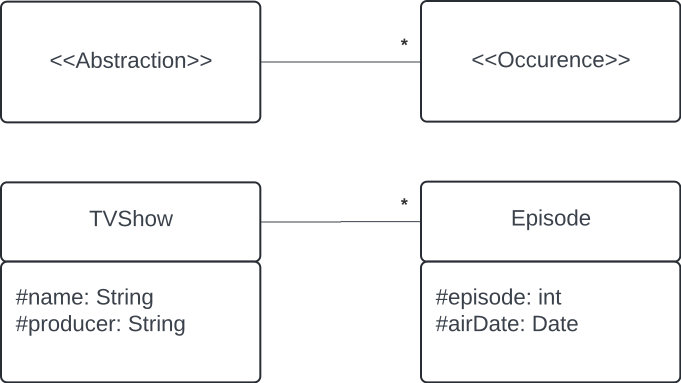
\includegraphics[scale=0.4]{part two/Objektorientierte Analyse/img/abstractionoccurence}
    \caption{Beispiel für das \textit{Abstraction-Occurence-Pattern}. (Quelle: eigene)}
    \label{fig:abstractionoccurence}
\end{figure}


\subsubsection*{Antipattern}
\begin{itemize}
    \item Alle Daten als Attribute einer Klasse modellieren (Zusammenhang von Klassen mit gleichen Daten wird nicht ausgedrückt)
    \item Vererbung (jedes Exemplar eine eigene Klasse)
\end{itemize}


\subsubsection*{Grenzen}
Kann nur sinnvoll eingesetzt werden, wenn die einzelnen Exemplare sinvoll unterschieden werden können, bspw. anhand einer \textbf{Identity}.



\subsection{Wechselnde Rollen (Player - Role)}

\subsubsection*{Problem}
\begin{itemize}
    \item ein Objekt kann in unterschiedlichen Kontexten verschiedene Verantwortlichkeiten und Beziehungen haben
    \item die Verantwortlichkeiten können sich ändern
\end{itemize}

\subsubsection*{Lösung}
\begin{itemize}
    \item Verantwortlichkeiten aus dem Objekt (\code{Player}) nehmen
    \item Verantwortlichkeiten in Objekte (\code{Role}) auslagern
    \item Konkrete Rollen erben von einer Rollensuperklasse
\end{itemize}

\subsubsection*{Beispiel}
s. Abbildung~\ref{fig:playerrole}

\begin{figure}
    \centering
    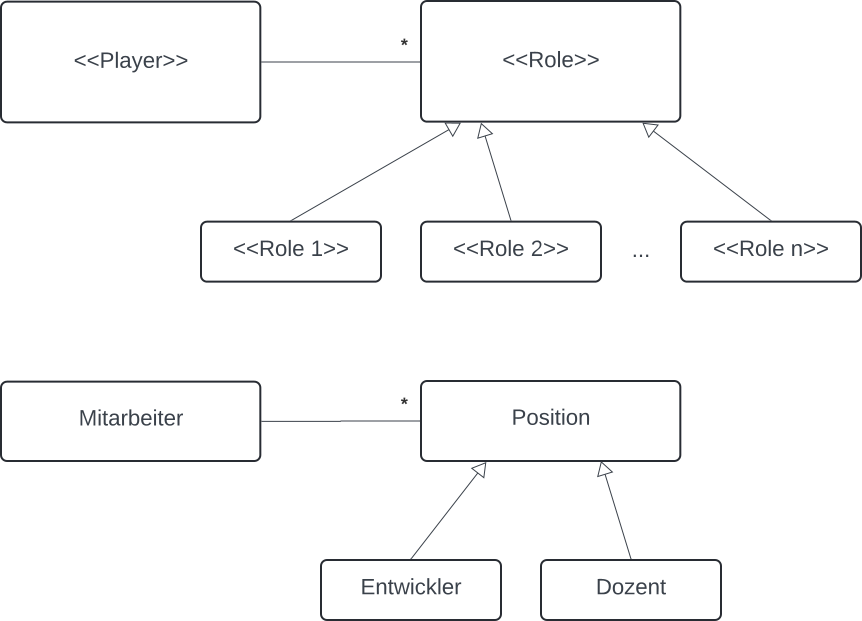
\includegraphics[scale=0.4]{part two/Objektorientierte Analyse/img/playerrole}
    \caption{Beispiel für das \textit{Player-Role-Pattern}. (Quelle: eigene)}
    \label{fig:playerrole}
\end{figure}


\subsubsection*{Antipattern}
\begin{itemize}
    \item Vererbung (eine Klasse identifiziert sich über den Typ der Rolle)
\end{itemize}


\subsection{Allgemeine Hierarchie (General Hierarchy, Kompositum)}

\subsubsection*{Problem}
\begin{itemize}
    \item Objekte können hierarchisch angeordnet sein
    \item Jedes Objekt kann maximal einem Objekt untergeordnet sein
    \item manche Objekte dieser Hierarchie können keine untergeordneten Objekte haben
\end{itemize}

\subsubsection*{Lösung}
\begin{itemize}
    \item Klassen werden von einer Superklasse \code{Node} abgeleitet
    \item Klassen, die andere Klassen referenzieren können, sog. \code{SuperiorNode}s, besitzen Referenzen auf \code{Node}s
    \item Klassen, die keine anderen Klassen referenzieren können, sind \code{NonSuperiorNodes}s
\end{itemize}

\subsubsection*{Beispiel}
s. Abbildung~\ref{fig:generalhierarchy}

\begin{figure}
    \centering
    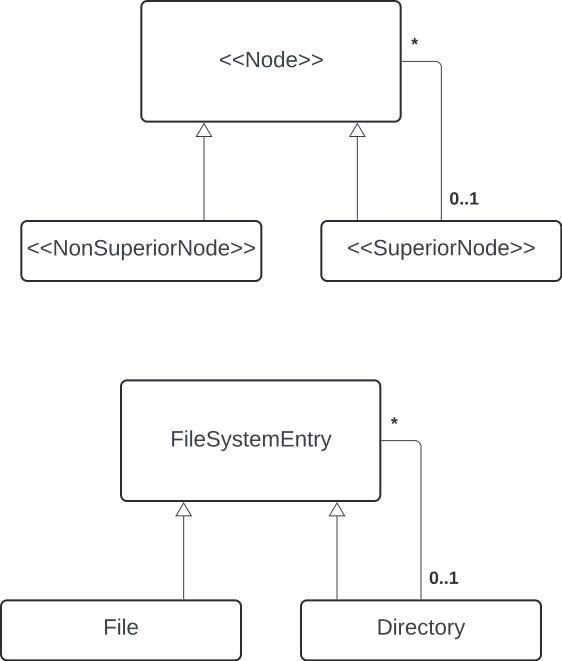
\includegraphics[scale=0.4]{part two/Objektorientierte Analyse/img/generalhierarchy}
    \caption{Beispiel für das \textit{General-Hierarchy-Pattern}. (Quelle: eigene)}
    \label{fig:generalhierarchy}
\end{figure}


\subsubsection*{Antipattern}
\begin{itemize}
    \item Vererbung: Die Vererbung beschreibt \textit{kann-verwendet-werden-als} oder auch \textit{ist-ein}, was bei einem Kompositum aber nicht immer zutrifft.
\end{itemize}


\begin{tcolorbox}
    \blockquote[{\cite[28, Hervorhebung eigene]{Wed09b}}]{
        Beim Muster \textit{Allgemeine Hierarchie} wird die Hierarchie von Objekten modelliert, nicht die Hierarchie von Klassen.
    }
\end{tcolorbox}


